\chapter{科学中的测量：单位与仪器}\label{ch:g6:measurement-in-science}

木匠、医生与天文学家走进各自的工作日：
一人量书架，一人量体温，一人测火星的漫游轨迹。三人
都依赖同一套默默运转的机制 --- 约定的单位、
可靠的仪器和仔细的读数。今年物理开始真正走向定量，
因此我们先打磨之后每一章都要依靠的
工具。

\section{从感觉到数值}

五年的实验教给我们一条规律：眼睛和双手
凭感觉去猜，仪器作出判断。尺子对照“看起来更长”；天平
对照“看起来更重”；温度计对照“觉得冷”。每一次，
仪器的结论都是\emph{带单位的数} ---
这一“数加单位”的组合可以传递、比较，任何人都能核查，
这是任何感觉都做不到的。

\begin{definition}[测量一个量]\label{def:g6:measurement-in-science:measuring}
\emph{测量}\index{测量}一个量 --- 长度、质量、
时长、温度 --- 就是数它里面约定的
\emph{单位}\index{单位}能放进去几次，借助为此而设计的仪器完成。
测量结果总是写成一个数，并且\emph{连同}其单位：
\qty{28.5}{cm}、\qty{450}{g}、\qty{37.2}{\celsius}。只写数字不写单位，只是传言；
数加单位，才算测量。
\end{definition}

\begin{example}[漏写单位的代价]\label{ex:g6:measurement-in-science:missing}
“加面粉 3。”克？勺？杯？蛋糕的成败就
系于漏掉的那个字。真实的事故，往往由漏写或
混淆单位引起——飞行员曾因把千克与磅弄混，
在飞行途中耗尽燃料。专业人员每次都写出单位，
毫无例外；从本章起，我们也这样做。
\end{example}

\section{世界通用的单位}

\begin{definition}[科学家的入门工具包]\label{def:g6:measurement-in-science:units}
世界已就常用单位达成一致，每一类量各有一套：
\begin{enumerate}
  \item 长度：\emph{米}（\unit{m}），及其倍数单位：
        千米（$\qty{1}{km} = \qty{1000}{m}$）、厘米
        （$\qty{100}{cm} = \qty{1}{m}$）和毫米
        （$\qty{1000}{mm} = \qty{1}{m}$）；
  \item 质量：\emph{千克}（\unit{kg}），连同克
        （$\qty{1}{kg} = \qty{1000}{g}$）和毫克
        （$\qty{1000}{mg} = \qty{1}{g}$）；
  \item 时间：\emph{秒}（\unit{s}），及分钟
        （$\qty{1}{min} = \qty{60}{s}$）和小时
        （$\qty{1}{h} = \qty{60}{min} = \qty{3600}{s}$）；
  \item 温度：摄氏度（\unit{\celsius}）；
  \item 液体的体积：升（\unit{L}），
        下一章我们将学习如何量取它。
\end{enumerate}
\end{definition}

\begin{example}[像科学家一样换算]\label{ex:g6:measurement-in-science:convert}
单位换算就是在十进制的阶梯上行走。
$\qty{2.35}{m}$ 换算成厘米：乘以 $100$ --- 小数点
向右移动两位，得 \qty{235}{cm}。$\qty{4500}{g}$ 换算成
千克：除以 $1000$，得 \qty{4.5}{kg}。时间是这个家族中的“叛逆者” ---
它的进位是 $60$，不是 $10$：$\qty{2.5}{min}$ 并不是
$250$ 秒，而是 $2 \times 60 + 30 = \qty{150}{s}$。请尊重
这位“叛逆者”。
\end{example}

\begin{remark}[谁在守护米的标准？]\label{rem:g6:measurement-in-science:guard}
两百年间，世界上的“米”是一根贵金属杆，
藏在欧洲某大都市附近一座戒备森严的金库里，而千克则是
它旁边一只闪亮的圆柱体：各国的尺子和砝码
都是复制再复制而来。如今，守卫已经
退役了：米和它的“同伴”现在都由
大自然本身不变的事实来定义 --- 光与原子内部的
“时钟”，因此地球上任何设备齐全的实验室（或
地球之外！）都能精确地重新复现它们。单位是人类
最长久的和平约定。
\end{remark}

\begin{omfigure}
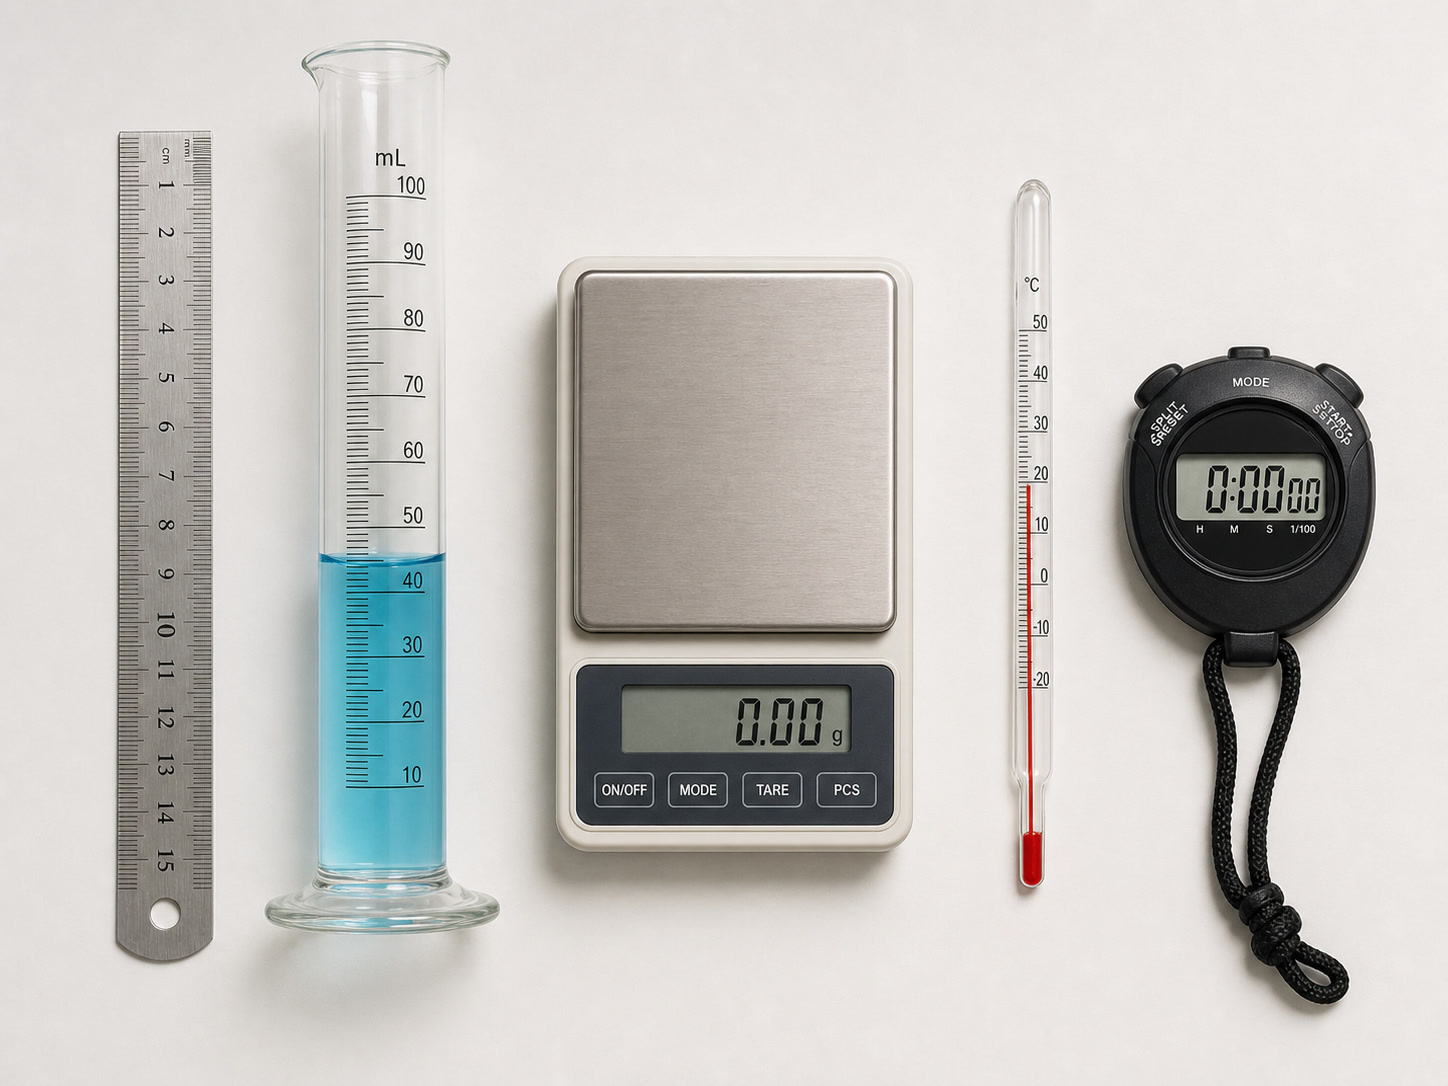
\includegraphics[width=0.55\linewidth]{images/book1/ai/g6-measurement-instruments.jpg}

{\small 测量工具箱：长度、体积、质量、温度和时间，每一类量都有自己的仪器和单位。}
\end{omfigure}

\section{正确使用仪器}

\begin{method}[读取任何带刻度的标尺]\label{met:g6:measurement-in-science:read}
尺子、温度计、量杯和表盘：
同一种技能就能读懂全部。
\begin{enumerate}
  \item 求出\emph{刻度值}：任取两个相邻的
        数字刻度线，相减，再除以它们之间的
        小格数 --- 以每厘米标数字、分十小格的尺子为例，
        每厘米分成十小格，每小格为
        $1 \div 10 = \qty{0.1}{cm}$，即一毫米；
  \item 视线正对刻度（斜看会让读数
        发生偏移）；
  \item 从最后一个数字刻度往后数：$7$ 和 $3$ 个
        小格，即 $7.3$；
  \item 写出\emph{带单位的数}。
\end{enumerate}
\end{method}

\begin{omfigure}
\begin{tikzpicture}[scale=0.85]
  \draw[thick] (0.4,0.6) -- (10.8,0.6);
  \foreach \x/\l in {0.8/5, 3.0/6, 5.2/7, 7.4/8, 9.6/9} {
    \draw[thick] (\x,0.6) -- (\x,1.35);
    \node[above, font=\small] at (\x,1.4) {\l};
  }
  \foreach \i in {1,...,9} {
    \draw (0.8+\i*0.22,0.6) -- (0.8+\i*0.22,1.0);
    \draw (3.0+\i*0.22,0.6) -- (3.0+\i*0.22,1.0);
    \draw (5.2+\i*0.22,0.6) -- (5.2+\i*0.22,1.0);
    \draw (7.4+\i*0.22,0.6) -- (7.4+\i*0.22,1.0);
  }
  \draw[-Stealth, very thick, omThm] (5.86,2.1) -- (5.86,1.15);
  \node[above, font=\small, omThm] at (5.86,2.15)
    {此处：$7$ 和 $3$ 个小格，$= 7.3$};
  \node[below, font=\small] at (5.6,0.3)
    {每个单位十小格，因此每小格代表 $0.1$};
\end{tikzpicture}

{\small 读懂刻度尺：先弄清一小格代表多少，
再从最后一个带数字的刻度往后数。}
\end{omfigure}

\begin{method}[估测、测量、判断]\label{met:g6:measurement-in-science:estimate}
专业人员从不贸然测量：
\begin{enumerate}
  \item \emph{估测}在先——“这张桌子大约两
        米”；
  \item \emph{选择}量程和刻度与任务相配的仪器
        （量一枚邮票用直尺，量走廊用卷尺，称面粉用厨房秤，
        称人的体重用体重秤）；
  \item \emph{测量}，按照读数规则进行；
  \item \emph{判断}：结果与估测是否大体相符？
        若一张桌子量得 \qty{21.3}{m}，
        桌子并没有长大——是你读错了，差了十倍，
        而估测正好把它揪了出来。
\end{enumerate}
估测是你的安全网：小数点点错位时，它会先把错误抓住，
免得错误先让你吃亏。
\end{method}

\begin{example}[慎重选择]\label{ex:g6:measurement-in-science:choose}
要称一封待寄的信，体重秤毫无用处——
这封信的 \qty{18}{g} 落在刻度之间，不见了踪影；厨房秤
以克为一格，恰好称准。要为
$100$ 米短跑计时，厨房钟表的分针刻度毫无用处；
秒表以百分之一秒计数。两者都谈不上“更好”，
各有各的适用范围，由量程和
最小刻度所决定。
\end{example}

\section{诚实的数值}

\begin{remark}[刻度之间]\label{rem:g6:measurement-in-science:between}
真实的指针偏爱停在刻度之间。此时，诚实有两个层次：
至少要写出相邻的两个刻度——“介于 $7.3$ 和
$7.4$ 之间，更接近 $7.3$”；更好的做法是再估读一位，
即“约 \qty{7.32}{cm}”。诚实所禁止的，是
编造精度：在毫米刻度上读出 \qty{7.3214}{cm}，
这纯属披着白大褂的虚构。仪器的刻度决定了它
所能保证的精确程度。
\end{remark}

\begin{example}[多测一次，更可信]\label{ex:g6:measurement-in-science:repeat}
三位朋友用同一块秒表测同一辆玩具车的运动时间：
\qty{4.6}{s}、\qty{4.8}{s}、\qty{4.7}{s}。没有人出错——
只是手指按下和松开时相差一丝。微小的离散是
实际测量中的正常波动。明智的做法是：多次重复测量，
观察读数是否集中，不轻信任何一个孤立的数字，
尤其是自己读出的那一个。
\end{example}

\section{练习}

\begin{exercise}[$\star$]\label{exo:g6:measurement-in-science:1}
为每个量填上合适的单位：门高 $2$
\dots\ ；硬币的质量是 $8$ \dots；一节课的时长是
$55$ \dots；发烧时体温为 $39$ \dots。
\end{exercise}

\begin{exercise}[$\star$]\label{exo:g6:measurement-in-science:2}
换算：\qty{3.2}{m} 化为 \unit{cm}；\ \qty{750}{g} 化为 \unit{kg}；\
\qty{4}{min} 化为秒；\ \qty{5600}{m} 化为 \unit{km}。
\end{exercise}

\begin{exercise}[$\star$]\label{exo:g6:measurement-in-science:3}
为什么时间是单位家族中的“叛逆者”？把 \qty{3.5}{min} 换算成秒
——并说明若沿用十进制的“阶梯”换算，
会得到怎样的错误答案。
\end{exercise}

\begin{exercise}[$\star$]\label{exo:g6:measurement-in-science:4}
一只量杯每隔 \qty{100}{mL} 标一个数字，数字之间
有五个小格。一小格代表多少？果汁液面
在 $300$ 刻度上方两小格处——果汁有多少毫升？
\end{exercise}

\begin{exercise}[$\star$]\label{exo:g6:measurement-in-science:5}
每项任务各用哪种仪器？为什么：称一小撮
酵母；\ 数心跳并计时；\ 量这一页纸的宽度；\ 量
操场的长度？
\end{exercise}

\begin{exercise}[$\star$]\label{exo:g6:measurement-in-science:6}
娜迪亚量她的铅笔，得到 \qty{17.4}{m}。在
\cref{met:g6:measurement-in-science:estimate}中，哪一道安全网本应拦下这个错误，
真实值可能是多少？
\end{exercise}

\begin{exercise}[$\star$]\label{exo:g6:measurement-in-science:7}
温度计的液柱停在 $18$ 与 $19$ 刻度之间，
更接近 $19$。请给出一种诚实的报告方式，以及
一种应当避免的不诚实的报告方式。
\end{exercise}

\begin{exercise}[$\star$]\label{exo:g6:measurement-in-science:8}
同一次跑步的三次秒表读数：\qty{6.1}{s}、\qty{6.3}{s}、
\qty{6.2}{s}。有人出错了吗？明智的报告应当怎样写？
\end{exercise}

\begin{exercise}[$\star\star$]\label{exo:g6:measurement-in-science:9}
国外的一份食谱要求“四分之一磅黄油”。你的
厨房秤显示的是克，而一整磅约为
\qty{450}{g}。你应称出多少克？这件
小事说明了关于通用单位的什么道理？
\end{exercise}

\begin{exercise}[$\star\star$]\label{exo:g6:measurement-in-science:10}
一把直尺的第一厘米已经磨损，因此它的边缘从
$1$ 刻度处开始计算。以边缘为起点放置的邮票，在另一端读数为 $3.4$。
这枚邮票的实际宽度是多少？什么样的习惯能应对磨损的直尺？
\end{exercise}

\begin{exercise}[$\star\star$]\label{exo:g6:measurement-in-science:11}
全班用一把 \qty{20}{m} 的卷尺测量走廊两次：
结果分别为 \qty{18.25}{m} 和 \qty{18.35}{m}。老师记下
“\qty{18.3}{m}”。请解释她这样选择的理由，并结合
\cref{rem:g6:measurement-in-science:between}和
\cref{ex:g6:measurement-in-science:repeat}作答。
\end{exercise}

\begin{exercise}[$\star\star\star$]\label{exo:g6:measurement-in-science:12}
一则古老的故事：某国国王下令，把自己的脚长定为王国的长度
单位。试列出由此引发的两种实际灾难（可想想远方城镇的木匠，
以及国王日渐长大的儿子作为继承人的情形），并说明已弃用的金属杆
如何解决了这两个问题——
\cref{rem:g6:measurement-in-science:guard}如何解决了这两个问题——
并指出金属杆仍未解决、最终由自然界常数定下来的
那个问题。
\end{exercise}

\section{问题：仪器检查员}

\begin{problem}[{周末问题——与镇上的
仪器检查员共度的一天；秤、量杯与钟表接受检验；
学徒的笔记本}]\label{pb:g6:measurement-in-science:1}
每年，镇上的检查员都要检验商店和
学校的仪器。今天，你就是那位学徒，手持笔记本。

\medskip\noindent\textbf{第一部分——面包店的秤。}
检查员带有经过认证的标准砝码：\qty{500}{g}、
\qty{200}{g}、\qty{200}{g}、\qty{100}{g}、\qty{50}{g}。
\begin{enumerate}
  \item 她检查空秤的指针是否恰好指在
        零刻度上。为什么这必须是第一项检验？
  \item 她放上 \qty{500}{g} 和一个 \qty{200}{g} 的砝码。
        诚实的秤应显示多少？
  \item 指针却显示 \qty{680}{g}。这台秤是
        偏袒面包师还是顾客？请说明每次售货时谁会吃亏。
        每次售货时，卖家都要多赚一些钱。
  \item 她的砝码中哪些组合可用来检验读数
        \qty{750}{g}？请给出一种。
  \item 面包店的秤以 \qty{5}{g} 为最小分度。检查员能否用它
        检验一枚 \qty{2}{g} 的邮票？
        为什么不能？
\end{enumerate}

\medskip\noindent\textbf{第二部分——学校的量杯。}
\begin{enumerate}[resume]
  \item 量杯每隔 \qty{200}{mL} 标一个数字，数字之间
        有四格。每格代表多少？
  \item 水面比 \qty{600}{mL} 刻度高出一格。教师
        的记录写着“约 \qty{700}{mL}”。请评定该报告是
        诚实、过于含糊，还是虚构？
  \item 一名学生坐在矮凳上读数，视线远低于
        水面，读出的数值与
        检查员不同。违反了哪条读数规则？
  \item 检查员将量杯标称的 \qty{650}{mL} 水倒入
        一只经认证的量杯中，显示为 \qty{640}{mL}。学校的量杯
        偏差多少？这一偏差比它自身的一格
        更差还是更好？
\end{enumerate}

\medskip\noindent\textbf{第三部分——钟表与学徒的
结论。}
\begin{enumerate}[resume]
  \item 车站的钟以无线电报时信号为准进行核对：
        报时信号显示正午时，它显示 $12$ h $2$ min。快了
        还是慢了？相差多少？
  \item 若无人校正，一周后它会超前多少？
        （它每天超前的量相同。）
  \item 三家商店的钟在信号报时正午时分别显示 $12$ h $2$ min、$11$ h $58$ min，
        以及 $12$ h 整。检查员
        说：“这里取平均毫无意义——应逐一校正每只
        钟。”各需怎样修理？
  \item 傍晚，请在笔记本上写下检查员的三条黄金法则——
        一条关于零点，一条关于读数，一条关于单位——
        每条都用你自己的一句话表述。
\end{enumerate}
\end{problem}
